\chapter{自动驾驶运行时通信系统测试与分析}
本章在上一章实现了自动驾驶运行时通信系统的各功能模块的基础上,以验证本系统设计的可行性与准确性为目标,展开
对整个自动驾驶运行时通信系统进行功能性测试和非功能性测试。本章从测试环境、测试方法以及测试结果展开论述,并给出测试结果。

\section{测试环境}
本节是对测试环境的介绍,即自动驾驶运行时通信系统的运行环境。本系统支持在兼容Linux的操作系统上运行,并且支持在x86或ARM架构
的CPU上运行。本文测试选用个人笔记本对系统进行测试,具体配置如表6.1所示。
\begin{table}[htb]
  \centering\small
  \caption{测试环境配置}
  \label{tab:exampletable}
  \begin{tabular}{cc}
    \toprule
    硬件 & 配置信息 \\
    \midrule
    操作系统 & Ubuntu16.04.12\\
    处理器 & Intel Core i7-8550U, 1.80GHz $\times$ 8\\
    内存 & 16GB, DDR4 2400MHz\\
    硬盘 & 512GB\\
    \bottomrule
  \end{tabular}
\end{table}
    
\section{功能性测试}
根据需求分析中对通信单元模块和服务模块提出的功能性需求,本节对通信单元模块和服务模块展开功能性测试。
\subsection{通信单元模块测试}
对于通信单元模块的测试,编写一个仅包含发布者的任务(test\_pub\_task)和一个仅包含订阅者(test\_sub\_task)的任务,双方以话题/test进行通信,通信数据为C++中的std::string类型,
通信类型为使用共享内存进行进程间通信,发布者以20HZ的频率向订阅者发布随机消息。


测试结果如图\ref{pub_sub_test}所示,左侧为发布者所在任务的终端,右侧为订阅者所在任务的终端。从图中可以看出,订阅者全部正确接收到
发布者发布的所有消息。

\begin{figure}[H]
  \centering
  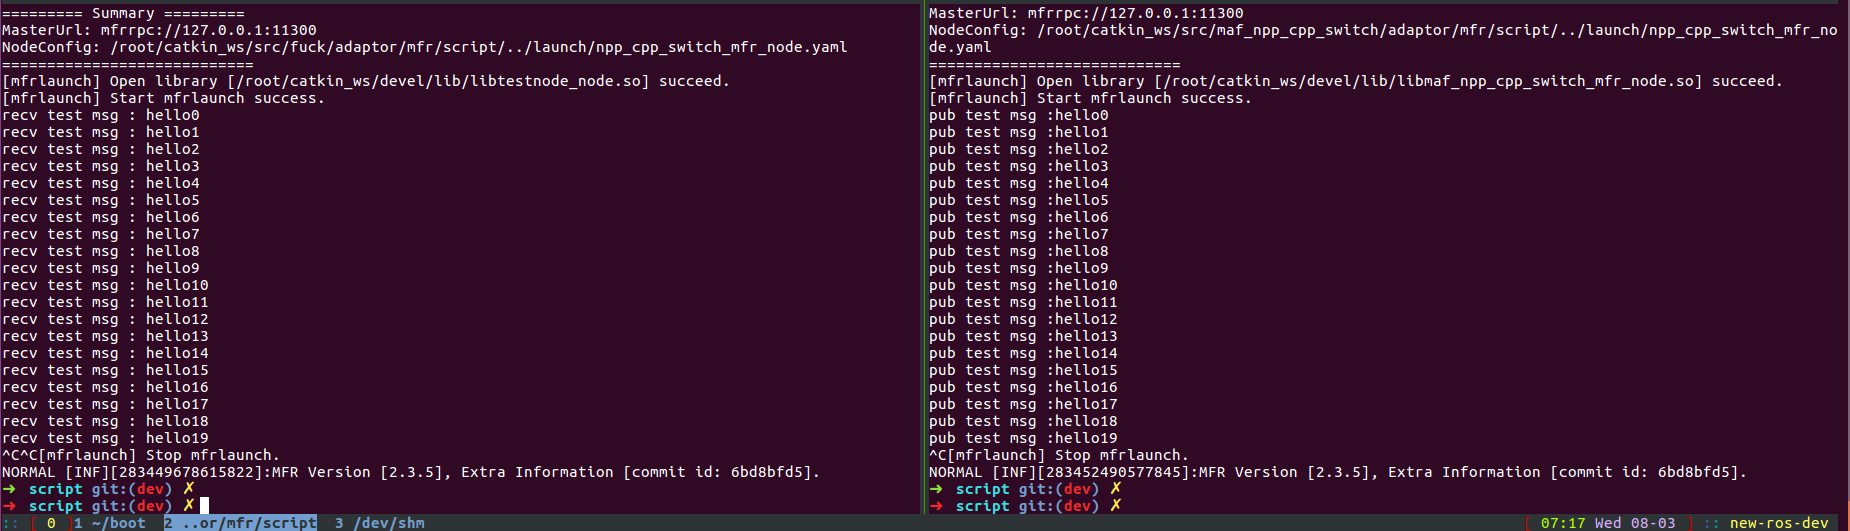
\includegraphics[width=0.95\textwidth]{pub_sub_test.png}
  \caption{任务模块类图}
  \label{pub_sub_test}
\end{figure}

\subsection{服务模块测试}
对于服务模块的测试,编写一个仅包含一个服务服务端的任务(test\_server\_task)和一个仅包含服务客户端(test\_client\_task)的任务,服务端提供名为/test的回射服务,客户端
向服务端发起请求,服务端将客户端的请求数据返回给客户端。


测试结果如图6.2所示。左侧为服务端所在任务终端,右侧为客户端所在任务的终端。从图中可以看出,服务端正确地返回了客户端的请求数据。
\begin{figure}[H]
  \centering
  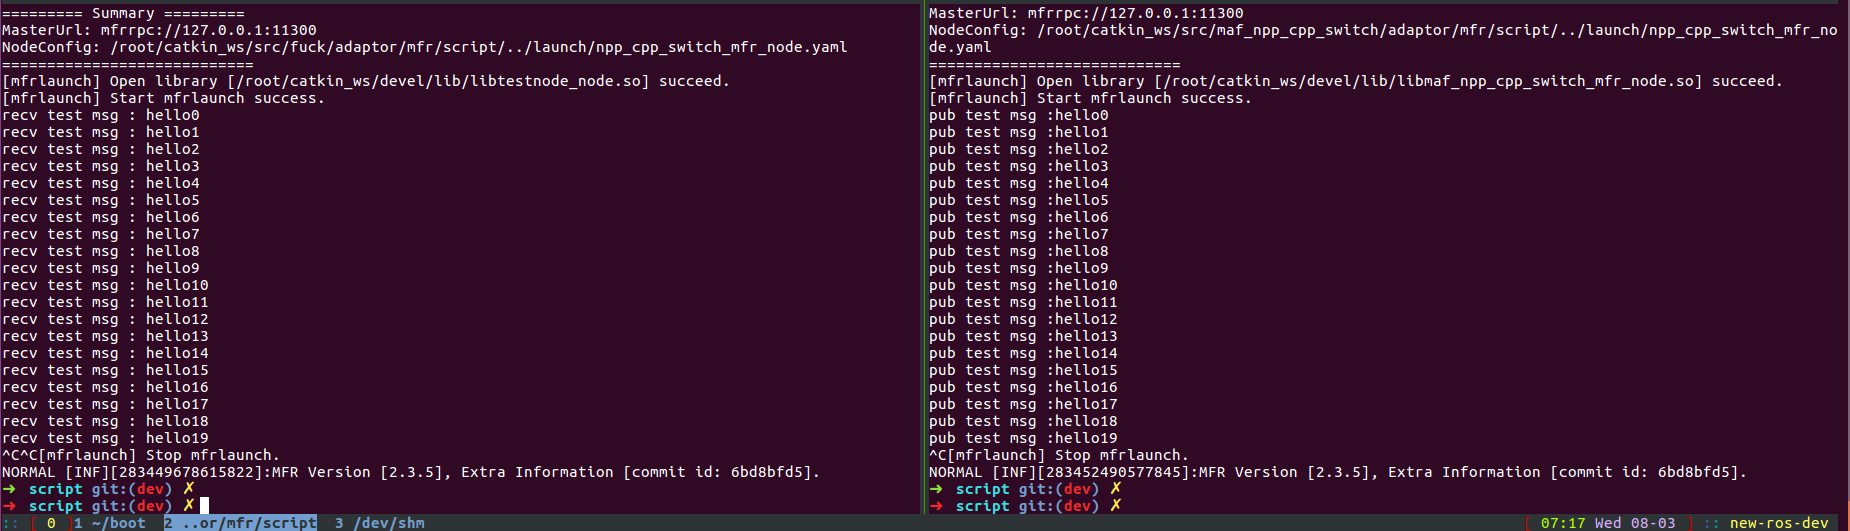
\includegraphics[width=0.95\textwidth]{pub_sub_test.png}
  \caption{任务模块类图}
  \label{pub_sub_test}
\end{figure}
\section{非功能性测试}
本系统的非功能性需求同功能性需求一样重要,本节对系统展开非功能性测试,着重于实时性测试。

\subsection{实时性测试}
实时性测试以端到端通信延迟作为衡量指标,测试系统的通信性能。实时性测试以消息大小、发布消息频率和订阅者数量
为变量,全面地对系统的通信性能进行测试。
\subsubsection{消息大小对通信延迟的影响}
本测试场景使用进程间通信的方式,在同一物理机内创建一个发布者和一个订阅者,将本系统共享内存通信(下文统一简写为SHM)、ROS的TCP通信(下文统一简写为ROSTCP)、ROS的UDP通信(下文统一简写为ROSUDP)和百度CyberRT共享内存通信(下文统一简写为CSHM)做通信性能
的对比。本测试固定发布者发布消息频率为10HZ,固定发送500条消息,消息大小分别选用1KB、1MB、4MB和8MB,给出四种通信方式的平均通信延迟、最小通信延迟以及
最大通信延迟。
\begin{table}[htb]
  \centering\small
  \caption{不同大小消息下各通信方式延迟}
  \renewcommand\arraystretch{1.2}
  \label{one_to_one}
  \begin{tabular}{ccccc}
    \toprule
    \multirow{2}{*}{通信方式} & \multirow{2}{*}{消息大小} & \multicolumn{3}{c}{延迟统计}\\
    % \cline{3-5}
     & & 平均延迟 & 最小延迟 & 最大延迟\\
    \midrule
    \multirow{4}{*}{SHM} & 1KB& 0.133935ms& 0.124816ms& 0.259271ms\\ & 1MB & 0.836192ms & 0.672181ms & 0.958912ms \\ & 4MB & 2.394001ms & 2.018293ms & 2.898237ms \\ & 8MB & 4.238182ms & 3.881239ms & 4.791298ms\\
    \hline
    \multirow{4}{*}{ROSTCP} & 1KB& 0.532441ms& 0.264735ms& 0.685397ms\\ & 1MB & 3.258292ms & 2.551780ms & 5.429340ms \\ & 4MB & 11.783733ms & 9.876647ms & 14.62529ms \\ & 8MB & 12.757952ms & 10.384041ms & 17.23690ms\\
    \hline
    \multirow{4}{*}{ROSUDP} & 1KB& 0.515512ms& 0.210117ms& 0.602012ms\\ & 1MB & 10.66662ms & 10.392843ms & 15.690852ms \\ & 4MB & 32.300212ms & 22.969457ms & 41.08326ms \\ & 8MB & 36.016137ms & 25.889108ms & 47.467454ms\\
    \hline
    \multirow{4}{*}{CSHM} & 1KB& 0.126589ms& 0.101587ms& 0.135296ms\\ & 1MB & 0.769871ms & 0.714389ms & 0.897123ms \\ & 4MB & 2.109284ms & 1.91240ms & 2.319872ms \\ & 8MB & 4.129837ms & 4.981398ns & 4.393987ms\\
    \bottomrule
  \end{tabular}
  \note{注:通信延迟数据包含数据序列化耗时}
\end{table}

表\ref{one_to_one}详细列出了各通信方式的通信延迟情况。从表中可以看出当消息大小在1KB时四种通信方式都可以将通信延迟
保证在1ms之内,但当消息大小达到MB级别时基于共享内存的进程间通信方式明显优于基于网络的进程间通信方式。SHM在通信延迟的表现
与CSHM在同一水平上,但SHM的通信延迟波动较CSHM更大。ROSTCP与ROSUDP在传输大数据量的消息时通信延迟明显上升,与SHM差距较大。值得注意的是ROS对于以UDP通信的方式,
单次传输消息大小的上限为1500KB,当实际消息大小超过1500KB时ROS内部将对消息进行分片并且接收时需要再次合并,且序列化与反序列化操作次数
也将增加,故ROSUDP的通信性能比ROSTCP更低。

\subsubsection{发布消息频率对通信延迟的影响}
本场景使用进程间通信的方式,在同一物理机内创建一个发布者和一个订阅者,将SHM、ROSTCP、和CSHM做通信性能对比。
本测试固定消息大小为4MB,固定发送1000条消息,发布频率分贝选用10HZ、20HZ和50HZ,给出四种通信方式的平均通信延迟、最小通信延迟以及
最大通信延迟。

\begin{table}[htb]
  \centering\small
  \caption{不同消息发布频率下各通信方式延迟}
  \renewcommand\arraystretch{1.2}
  \label{one_to_one}
  \begin{tabular}{ccccc}
    \toprule
    \multirow{2}{*}{通信方式} & \multirow{2}{*}{频率大小} & \multicolumn{3}{c}{延迟统计}\\
    % \cline{3-5}
     & & 平均延迟 & 最小延迟 & 最大延迟\\
    \midrule
    \multirow{3}{*}{SHM} & 10HZ& 2.429173ms& 2.101929ms& 2.981249ms\\ & 20HZ & 0.836192ms & 0.672181ms & 0.958912ms \\ & 50HZ & 2.394001ms & 2.018293ms & 2.898237ms \\
    \hline
    \multirow{3}{*}{ROSTCP} & 10HZ& 11.984234ms& 9.975642ms& 12.370449ms\\ & 20HZ & 8.958139ms & 4.623674ms & 12.128937ms \\ & 50HZ & 4.362920ms & 3.106624ms & 11.234283ms \\
    \hline
    \multirow{3}{*}{CSHM} & 10HZ& 0.126589ms& 0.101587ms& 0.135296ms\\ & 20HZ & 0.769871ms & 0.714389ms & 0.897123ms \\ & 50HZ & 2.109284ms & 1.91240ms & 2.319872ms \\
    \bottomrule
  \end{tabular}
  \note{注:通信延迟数据包含数据序列化耗时}
\end{table}

